\documentclass[12pt,a4paper]{article}

% ----------------------------
% Pacotes de formatação
% ----------------------------
\usepackage[sfdefault]{carlito}       % Fonte principal
\usepackage{graphicx}                 % Inserir imagens
\usepackage{amsmath}                  % Fórmulas matemáticas
\usepackage{enumitem}                 % Listas customizadas
\usepackage{csquotes}                 % Citações inteligentes
\usepackage{xurl}                     % URLs quebráveis
\usepackage{setspace}                 % Controle de espaçamento
\usepackage{xcolor} 				  % Define cores básicas
\usepackage[breaklinks,colorlinks,allcolors=blue,citecolor=black]{hyperref}
\usepackage{booktabs}
\usepackage{array} 
\usepackage{tabularx}
\usepackage{longtable}
\usepackage{booktabs}
\usepackage{caption}
\usepackage{multirow}

\usepackage[style=abnt]{biblatex} % Bibliografia ABNT 2023
\addbibresource{bibliografia.bib}                   % Arquivo .bib

\usepackage[top=30mm,bottom=20mm,left=30mm,right=20mm]{geometry}  % Margens A4

% ----------------------------
% Configurações gerais
% ----------------------------
\singlespacing     % Espaçamento simples para resumo e título
\setlength\parindent{1.25cm}  % Recuo de parágrafo

% ----------------------------
% Início do documento
% ----------------------------
\begin{document}
	
	% ----------------------------
	% Página de rosto
	% ----------------------------
	\thispagestyle{empty}
	\begin{center}
		
\includegraphics[keepaspectratio,height=1cm]{fapesp.png} \\[0.5cm]
		{\Large Fundação de Amparo à Pesquisa do Estado de São Paulo (FAPESP)\\
			Bolsa de Pós-Doutorado}
		
		\vspace{1cm}
		
		{\LARGE \textbf{Alterações ômicas centrais e periféricas induzidas pela quimioterapia e seus efeitos na indução de déficit cognitivo \textit{("chemobrain")}: potenciais novos biomarcadores}}
		
		\vspace{1cm}
		
		{\large Candidato: Dr. Arlindo C. M. Pereira \\ \vspace{0.1cm}
		Orientador: Prof. Dra. Sabrina F. S. Lisboa \\
		\vspace{0.2cm}
		Faculdade de Ciências Farmacêuticas de Ribeirão Preto (FCFRP) - USP} \\
		 \LaTeX  
	\end{center}
	
	\clearpage
	
	% ----------------------------
	% Resumo
	% ----------------------------
\begin{abstract}
\noindent O chemobrain é uma condição médica na qual o paciente que está sob quimioterapia apresenta declínio. Uma possível causa seria a indução da senescência celular no cérebro, neuroinflamação, aumento do estresse oxidativo, perda de integridade neuronal, diminuição da neurogênese e neuroplasticidade, entre outros. Apesar do relativo bem entendimento dos processos fisiopatológicos subjacentes ao fenômeno, o entedimento dos mecanismos moleculares por trás dos mesmos dificulta identificar o que é causa e o que é consequência. Este projeto tem como objetivo principal idenficicar as causas primárias do chemobrain a nível molecular, possibilitando abordagens de tratamento mais eficiente. Para isso, será feito uma meta-análise usando Python e R de dados ômicos ex vivo de diferentes bases de dados, como Gene Expression Omnibus, Array Express e Proteome Xchange (transcriptoma, proteômica, microbioma). Os resultados serão comparados com a literatura através de data-mining. Finalmente, as alterações que se mostrarem mais consistentemente presentes e apresentarem maior potencial translacional como biomarcadores serão validadas em estudos in vivo utilizando camundongos C57Bl/6. A validação será feita primeiramente buscando detectar as alterações selecionadas em técnicas como PCR, Western Blot, entre outras, a depender de sua natureza; então, será feita uma avaliação da correlação dessas alterações com a magnitute do déficit cognitivo em ensaios comportamentais.
		
\paragraph{Palavras-chave:} Neurofarmacologia; Senescência; Declínio cognitivo; Ciências ômicas; Bioinformática.
\end{abstract}
	
	\clearpage
	
	% ----------------------------
	% Corpo do texto
	% ----------------------------
	\doublespacing   % Espaçamento 2x no corpo do texto

\section{Introdução e justificativa} \indent
	
De acordo com a Organização Mundial da Saúde, o câncer é o conjunto de doenças responsável por uma a cada seis mortes no mundo \cite{WorldHealthOrganization2022}. O avanço na pesquisa do câncer e o desenvolvimento de novos tratamentos nas últimas décadas têm aumentado a quantidade de pessoas que sobrevivem a este conjunto de doenças, e a sobrevida dos demais pacientes \cite{Gutmann2019}. Entretanto, entre 70\% e 75\% dos pacientes que passam por períodos prolongados de quimioterapia desenvolvem alterações cognitivas, condição chamada de CICI (chemotherapy-induced cognitive impairment), CRCI (chemotherapy-related cognitive impairment ), ou “chemobrain” \cite{Rao2022}. \\
	
Alterações cognitivas após a quimioterapia têm sido relatadas na literatura desde aproximadamente a década de 1970 \cite{Hinton1972,Levine1978, Meadows1976}, embora esse fenômeno tenha sido avaliado de forma controlada em relação ao câncer somente no início da década de 1980 \cite{Davis1987, Oxman1980, Silberfarb1980}. Só a partir de 2000 começaram a aparecer termos específicos para caracterizar o quadro, entre eles “chemobrain”, “chemofog”, “chemotherapy-induced cognitive impairment”, entre outros. \\
	
Pacientes com chemobrain podem apresentar diminuição de aprendizado, atenção, memória, função executiva e velocidade de processamento. Embora em muitos casos o efeito seja reversível após o fim da quimioterapia, até 50\% dos pacientes apresentam chemobrain por longos períodos, de meses e até anos após o fim do tratamento. Há registros em estudos transversais da persistência do déficit cognitivo até mesmo 20 anos após o fim da quimioterapia em sobreviventes de câncer de mama \cite{Ren2019, Ren2019a}. Análises de ressonância magnética funcional mostram alterações estruturais – como alterações no volume e densidade de matéria branca e cinzenta – no cérebro dos pacientes, evidenciando uma base biológica para esse fenômeno \cite{Rao2022}. \\
	
Mesmo apesar das evidências demonstrando o chemobrain, tanto clínicas quanto experimentais, não há até o momento nenhuma forma de tratamento ou prevenção para a condição. A pesquisa do tratamento ao câncer, coerentemente sempre foi focada na sobrevivência dos pacientes. Hoje, porém, com aumento da sobrevida dos pacientes, e das taxas de sobrevivência, surge a necessidade de buscar não somente o tratamento contra o câncer em si, mas também na melhoria da qualidade de vida, visto que, com o envelhecimento natural da população mundial, é esperado que a prevalência do câncer, e consequentemente da quimioterapia e seus efeitos adversos, tendem a representar um problema de saúde pública maior. \\
	
Uma das possíveis razões para não existência de tratamentos é o não entendimento dos mecanismos que desencadeiam o fenômeno. Entender os mecanismos moleculares pode apontar os alvos, e consequentemente, possíveis abordagens de tratamento que poderiam ser utilizadas. O presente trabalho fornecerá informações sobre alterações ômicas causadas pela quimioterapia, e posteriormente estudará experimentalmente quais as principais dessas alterações estão mais relacionadas ao déficit cognitivo. Ao mesmo tempo que as informações podem ser úteis na inferência de possíveis tratamentos, poderá também indicar biomarcadores associados ao quadro. \newpage
	
	
\section{Objetivos}
	\textbf{Objetivo geral}
	
Avaliar as principais alterações ômicas associadas ao déficit cognitivo induzido por quimioterapia. \\
\\
	\textbf{Objetivos específicos}
\begin{itemize}
		\item Fazer uma meta-análise de dados ômicos disponíveis em bancos de dados especializados com o intuito de estudar as principais alterações ômicas observadas durante a quimioterapia no sistema nervoso, sangue e microbiota (proteômica, transcriptômica, microbioma, lipidômica);
		\item Comparar possíveis diferenças observadas entre natureza do sistema nervoso (central ou periférico), espécie, ou quimioterápico, de acordo com a disponibilidade de dados;
		\item Comparar as principais alterações ômicas observadas com as de outros fenótipos onde há déficit cognitivo;
		\item Validar as principais alterações selecionadas in vivo em animais tratados com quimioterápico utilizando técnicas como PCR (para alterações transcriptômicas) e Western Blot (proteômica);
		\item Correlacionar as alterações validadas com o grau de declínio cognitivo observado nos animais através de ensaios comportamentais (Novel Object Location/Recognition).
\end{itemize}	\newpage
	
\section{Material e métodos} \indent 

O projeto será dividido em três etapas principais: 1) Levantamento inicial das bases de dados; 2) Análise dos dados obtidos; 3) Validação experimental. O processo é esquematizado na Figura 1. 
	% Figura Metodologia
\begin{figure}[htbp]
		\centering
		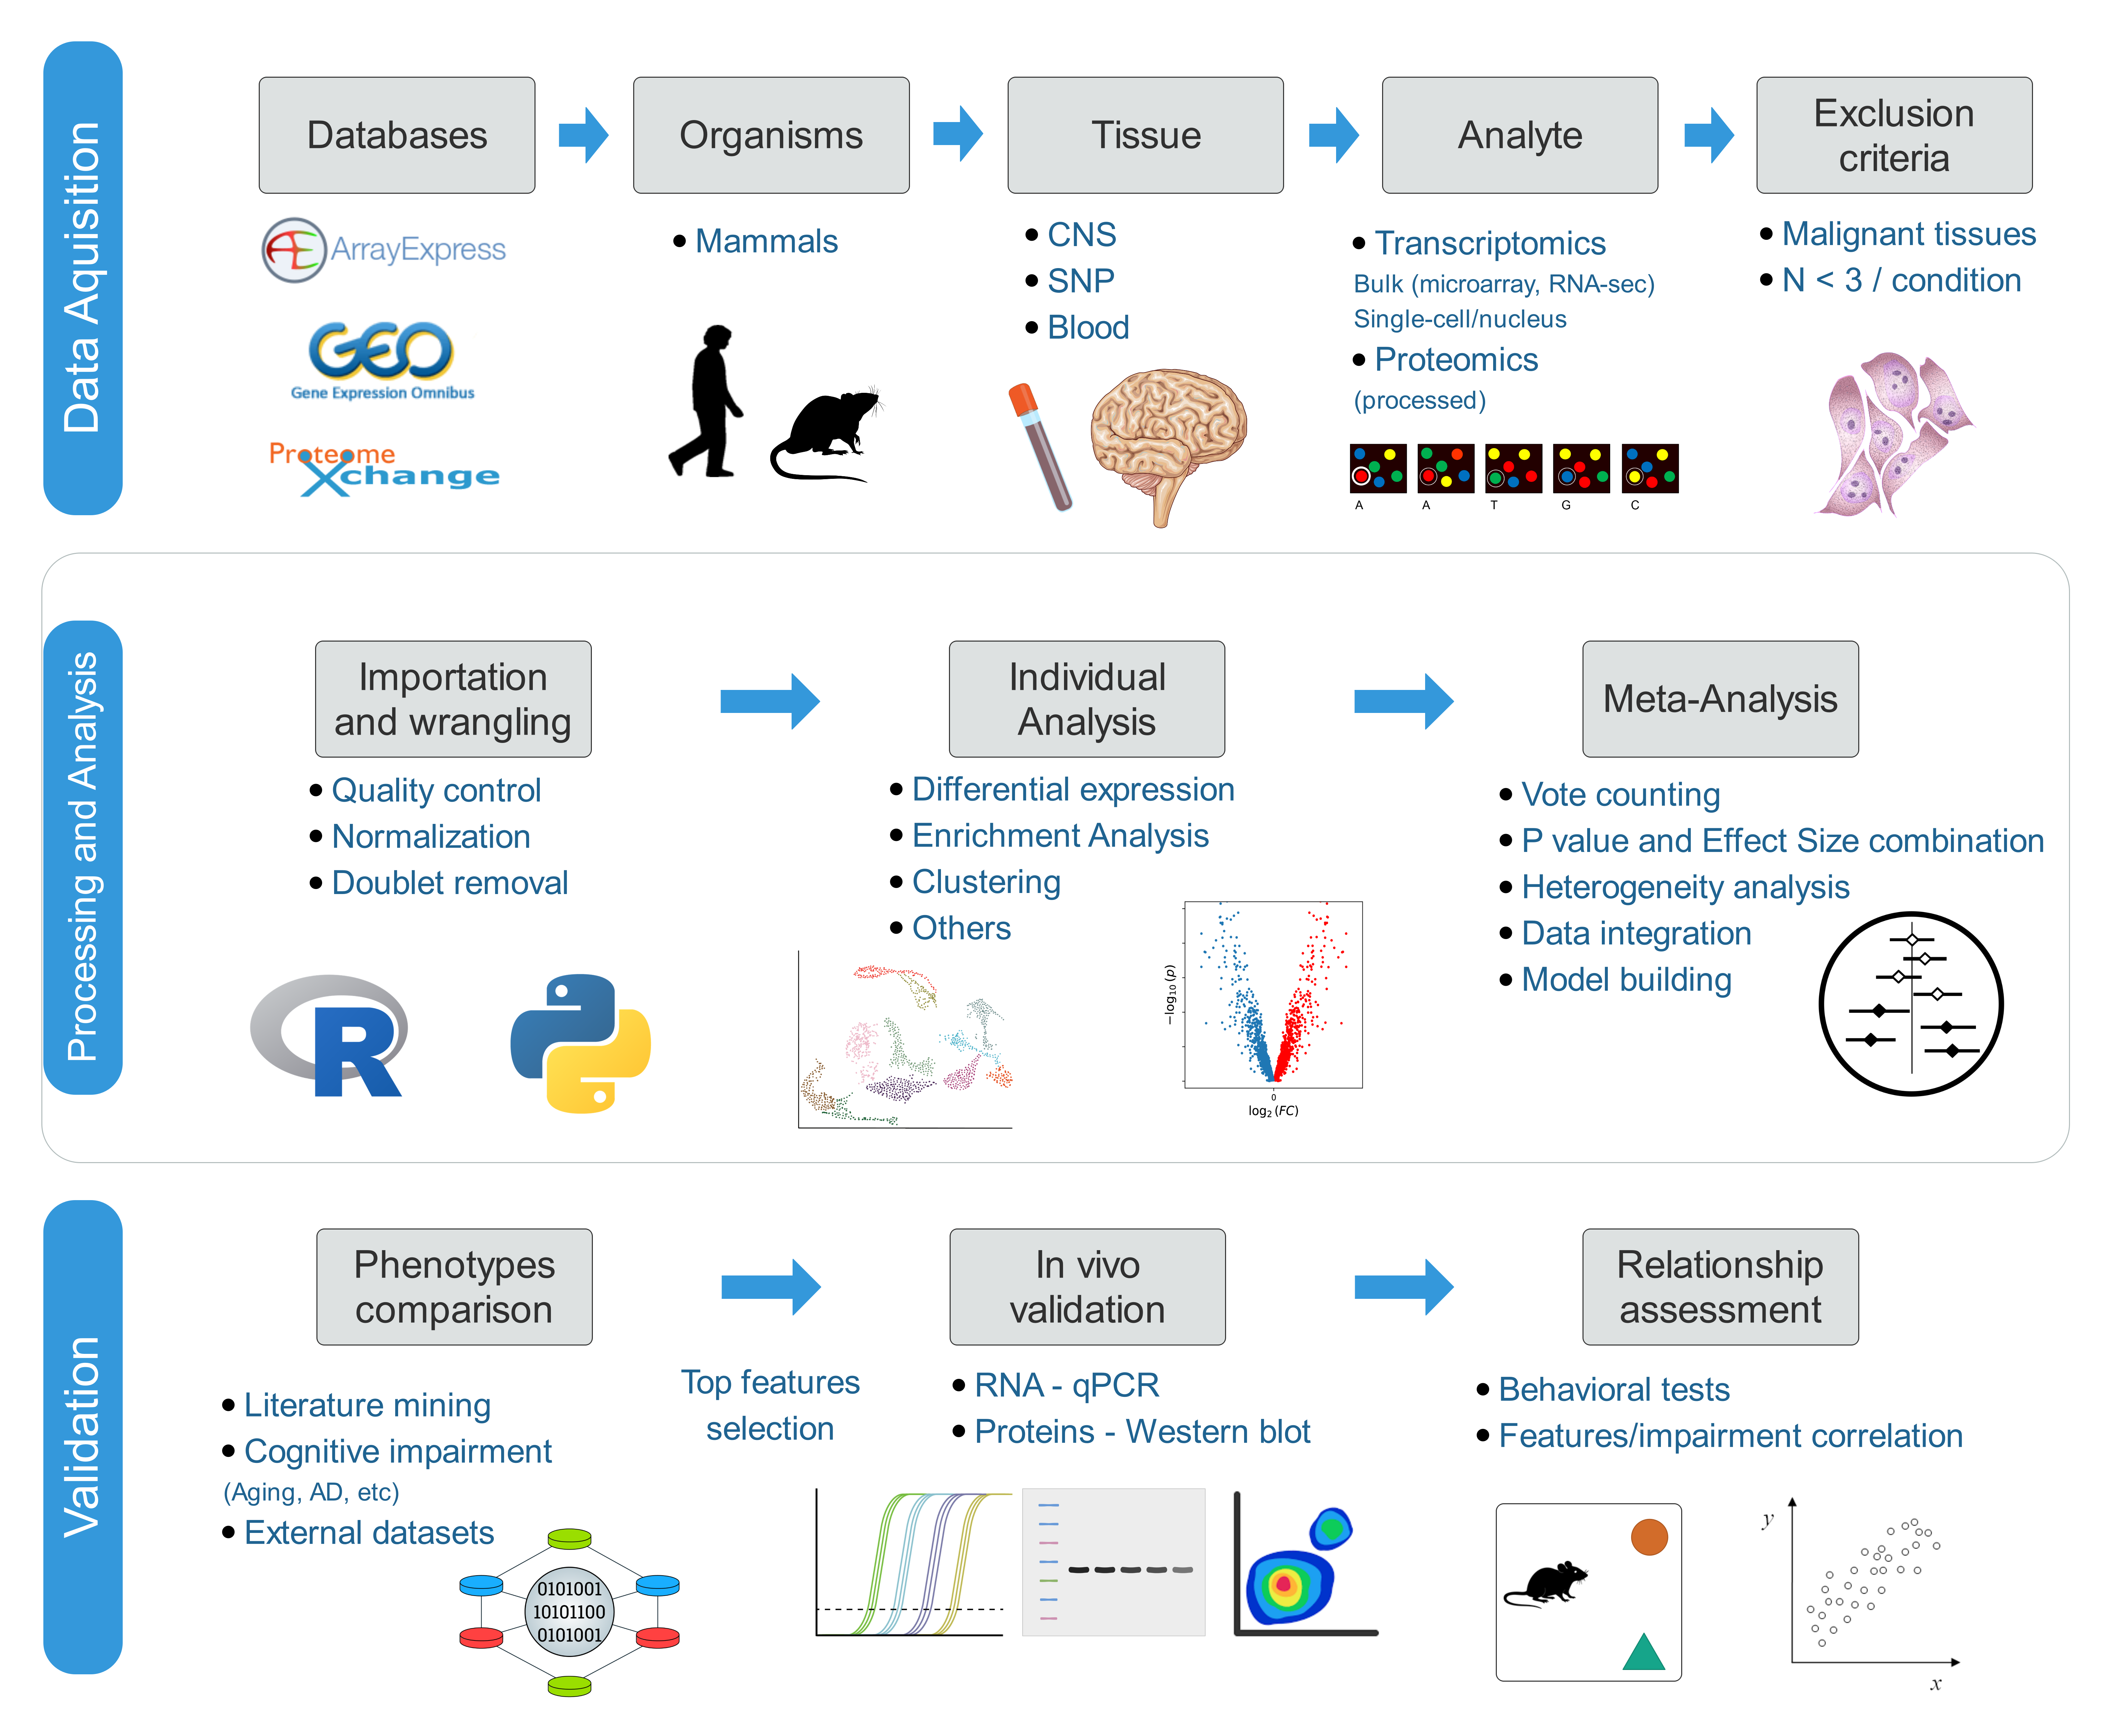
\includegraphics[height=12cm,keepaspectratio]{PD.png} % ou PD.pdf
		\caption{Esquema do projeto proposto.}
		\label{fig:PD}
\end{figure}

\subsection{Levantamento dos Dados}	\indent 

A pesquisa de dados brutos será feitas nas bases Gene Expression Ominubus (GEO) da Natinal Institute of Health, Proteome Xchange e Array Express, podendo ser adicionadas outras bases no decorrer do projeto se necessário. Para alterações no sistema nervoso diretamente relacionadas ao chemobrain (SNC) serão pesquisadas palavras-chaves como "Chemobrain", "Chemofog", "Chemotherapy-Induced Cognitive Impairment" e "Chemotherapy-Related Cognitive Impairment". \\
	
A fim de comparar alterações ômicas envolvidas na neurotoxicidade central com a neurotoxicidade periférica, pesquisadas também as keywords "Chemotherapy-induced Peripheral Neuropathic Pain" e "Chemotherapy-induced Peripheral Neuropathy". Adicionalmente, com o intuito de procurar alterações sistêmicas que possam ser utilizadas como biomarcadores, será feita uma busca geral "chemotherapy" com filtro de tecido: sangue/plasma. \\
	
Serão usados apenas resultados provenientes de mamíferos com N igual ou maior a 3 por condição, e não serão utilizados dados proveninentes diretamente de tecido tumoral (como linhagens celulares em cultura ou glioma). Não serão utilizados filtros de data ou de  qualquer outro tipo além dos aqui mencionados. Na Tabela 1 são mostrados alguns dadasets já coletados até o momento. \\
% Tabela Dados  
\begin{center}	
	\centering	\small	\begin{longtable}{p{0.5cm} p{2.5cm} p{3cm} p{3cm} p{2cm} p{3cm}}
	\captionsetup{justification=justified, width=\textwidth}
	\caption{Dados já coletados até o momento. AC-T: Ciclofosfamida+Paclitaxel+Doxorubicina; PFC: Pré-frontal córtex; VEs: Vesículas Extracelulares; FOLFOX: Leucoverina, Fluorouracil, Oxaliplatina; DRG: Dorsal-root ganglion.}  \\
	\toprule  
	N° & Tratamento & Organismo & Método e ID & Tecido & Referência \\  
	\midrule  
	\endfirsthead  
		1 & AC-T & Camundongos C57BL/6 fêmeas & RNA (bulk seq; GSE295281) & Hipocampo & Não publicado \\
		2 & AC-T & Camundongos C57BL/6 fêmeas & Proteômica (PXD017271) & Hipocampo & \cite{McElroy2020} \\
		3 & Doxorrubicina & Ratos Fischer machos & RNA (bulk seq; GSE236404) & Hipocampo (DG) & \cite{Budamagunta2024} \\
		4 & Cisplatina & Camundongos C57BL/6 fêmeas & RNA (single-cell; GSE216146) & Hipocampo & \cite{Kim2024} \\
		5 & Doxorrubicina & Camundongos C57BL/6 machos & RNA (bulk seq; GSE178812) & Hipocampo & \cite{Cavalier2021} \\		
		6 & Mitramicina  & Ratos Wistar machos & RNA (microarray; não depositado) & PFC & \cite{Asor2018} \\
		7 & PTX & Camundongos C57BL/6 (m/f) & RNA (bulk seq; não depositado)	 & PFC & \cite{Liang2020} \\
		8 & PTX & Pacientes & 16S rRNA (E-MTAB-13423) & Microbiota & \cite{Zhong2023} \\
		9 & PTX & Ratos Sprague-Dawley & 16S rRNA (E-MTAB-13426) & Microbiota & \cite{Zhong2023} \\
		10 & Doxorrubicina & Pacientes & Proteômica & Plasma (VEs) &  \cite{Koh2021} \\
		11 & FOLFOX & Pacientes & RNA (bulk seq GSE260661) & Leucócitos circulantes & \cite{Ju2024} \\
		12 & Cliclofosfamida & Camundongos DBA/2 com tumor & RNA (bulk microarray; GSE27422) & Leucócitos circulantes & \cite{Ju2024} \\
		13 & Cisplatina & Ratos Wistar machos e fêmeas & RNA (bulk seq; GSE281897)  & DRG & \cite{DaVitoriaLobo2024} \\
		14 & PTX & Camundongos C57BL/6 machos e fêmeas & RNA (bulk seq GSE240708) & DRG & \cite{Naratadam2024} \\
		15 & Vincristina & Camundongos C57BL/6 (sexo não especificado) & RNA (bulk seq; GSE125001) & DRG & \cite{Starobova2020} \\
		16 & Oxaliplatina e Cisplatina & Camundongos C57BL/6 (sexo não especificado) & (bulk seq; GSE125002) & DRG & \cite{Starobova2020} \\
		17 & PTX & C57BL/6 machos & RNA (bulk seq; GSE268185)  & Medula espinhal & \cite{Sierra2025} \\
		18 & Oxaliplatina & C57BL/6 machos e fêmeas & RNA (bulk seq; GSE253183) & Medula espinhal & \cite{Wang2024c} \\
		19 & Cisplatina & C57BL/6 machos & RNA (bulk seq; GSE154816)  & Medula espinhal (micróglias) & \cite{Navia-Pelaez2021} \\
	\bottomrule
	\end{longtable}
\end{center}
	
\subsection{Análises individuais e meta-análise} \indent
	
Adquiridos os dados, os mesmos serão analisados de acordo com sua natureza. Dados de microarray serão analisados no R com o pacote "limma", dados de RNA seq bulk serão analisados no R com o pacote "DESeq", dados provenientes de experimento single-cell ou single-nucleus serão analisados no Python devido ao tamanho dos datasets. Alguns códigos já estão escritos, sendo encontrados no github do autor (https://github.com/arlindomatias/projects). Após feitas as análises individuais, será feita uma meta-análise geral, por métodos como vote-counting, pooling de effect-sizes e valores p, entre outros \cite{Mosquera2023}.
	
\subsection{Text Mining} \indent
	
Tendo sido obtidos as principais alterações ômicas induzidas por quimioterapia, serão selecionados aquelas alterações significativas que tenham maior relação com o déficit cognitivo. Para isso, será feito text mining da literatura das principais alterações com outros fenótipos onde há déficit cognitivo, comparando os principais biomarcadores com os features selecionados nas análises anteriores. Para o text mining será utilizado o método descrito em \cite{Kveler2018}
Os principais candidatos serão finalmente validados em animais. \\
	
	
\subsection{Animais e Aspectos Éticos} \indent
	
Serão usados camundongos (Mus musculus) C57BL/6 machos adultos (9 semanas no início dos testes). Os animais serão adquiridos do biotério central da Universidade de São Paulo, campus Ribeirão Preto, mantidos em cabines ventiladas (n = 3-5/caixa) sob controle de temperatura (24 ± 1 ◦ C), ciclo claro/escuro (12h/12h, 6 às 18 h), e umidade (50\%-55\%), com acesso a comida (Nuvital, Nuvilab, Brazil) e água filtrada ad libitum. O uso dos animais será submetido ao CEUA da FCFRP ainda antes dos testes de validação (Tabela 2). \\
		
	
\subsection{Tratamento e Delineamento Experimental} \indent

Para indução do chemobrain será utilizado como protótipo de quimioterápico o paclitaxel (PTX), administrado por via intraperitoneal à 15 mg/kg, diluído em Cremophor EL:Etanol:Salina (1:1:18), numa concentração final de 2 mg/mL. A injeção será feita seis vezes, sendo feita três injeções em dias alternados, seguido de dois dias de recuperação, e mais três injeções em dias alternados (Figura 2A). \\
	
Haverá um grupo controle tratado apenas com veículo e um grupo tratado com PTX. O n amostral foi calculado no R usando o pacote "pwr". Como o objetivo do estudo é correlacionar os marcadores ao grau de comprometimento cognitivo, o n amostral foi calculado em relação à correlação (Pearson; r = 0.5; sig.level = 0.05; poder = 0.8). A análise indicou o n de 28 animais tratados com PTX, sendo esse valor também adotado para o grupo controle. \\
	
\subsection{Testes Comportamentais} \indent
	
A sequência de testes será feita de logo após o tratamento (Figura 2A). O teste de campo aberto será feito em uma arena circular de 30 cm de diâmetro e 40 cm de altura, durante 5 minutos de filmagem. O teste do campo aberto não avaliará a performance cognitiva propriamente dita, porém dá resultados importantes sobre a toxicidade geral nos animais), sendo importante para detectar animais mais debilitados ao tratamento e filtrá-los a fim de evitar viés da toxicidade geral.\\
	
Um dia após o campo aberto será feita a fase de aquisição (5 min.) do teste de localização de objeto no mesmo aparato, usando dois objetos idênticos; duas horas depois foi feita a fase de localização, trocando a posição de um dos objetos. A fase de localização do teste de localização de objeto também funciona como fase de aquisição do teste de reconhecimento de objeto novo. Duas horas depois, um dos objetos será trocado para avaliar o reconhecimento de objeto de curto prazo durante cinco minutos. O reconhecimento de objeto será avaliado também no longo prazo, trocando novamente o objeto novo e avaliando a interação dos animais um dia depois do teste de reconhecimento de curto prazo. \\
	
Os parâmetros avaliados no campo aberto de forma automática (Anymaze 7.2) foram distância percorrida e atividade no centro da arena. Na localização e reconhecimento de objeto será calculado o índice de discriminação (ID) como a razão entre a diferença entre o tempo de exploração do objeto modificado (M) e familiar (F), sobre a soma do tempo de exploração de ambos os objetos: ID = (M – F) / (M + F). 
	
	
	
\subsection{Ensaios ex vivo} \indent
	
A partir dos resultados obtidos de alterações ômicas relacionadas ao chemobrain, serão selecionados 5 sondas de qPCR e 3 anticorpos para Western Blot, correspondentes às maiores alterações de expressão gênica e abundância proteica, respectivamente. 

A preferência da validação por biomoléculas de RNA e proteínas é dada devido à maior disponibilidade de dados desta natureza. Porém, a depender do tempo, recursos disponíveis e resultados obtidos nos levantamentos, poderá ser feita validação de outras alterações ômicas, como lipidômica (com caracterização feita por HPLC-MS/MS) e microbiômica (metagenômica). Alterações a nível de populações celulares, caso sejam evidenciados, poderão ser avaliadas por citometria.
	
\subsection{Data Analysis} \indent
	
Para a análise de dados dos testes de validação ex vivo e in vivo, os resultados serão inicialmente avaliados em relação a homocedasticidade e normalidade da distribuição respectivamente pelos testes de Welch e Shapiro-Wilk. Em caso de dados paramétricos, serão posteriormente analisados com os seguintes testes: teste T e Pearson (correlação). Para dados não paramétricos será utilizado teste U e Spearman (correlação). Em casos de comparações entre grupos com dois fatores, será realizado 2W-ANOVA. O effect size será apresentado por valores t, U, r, rho ou cohen’s d a depender do teste.
	
	
\section{Plano de Trabalho e Resultados Preliminares} \indent
	
O processo geral do trabalho é mostrado na Figura 1, como descrito na metodologia. O cronograma proposto é mostrado abaixo. \\
	
\begin{table}[htbp]
	\centering
	\caption{Cronograma de atividades por trimestre} % legenda acima
	\begin{tabular}{llllllll}
		\hline
		\multicolumn{1}{c}{\multirow{2}{*}{Atividade}} & \multicolumn{7}{c}{Trimestre} \\
		\multicolumn{1}{c}{}                           & 1  & 2  & 3  & 4  & 5 & 6 & 8 \\
		\hline
		Levantamento dos dados                         & x  & x  & x  &    &   &   &   \\
		Comitê de ética                                & x  & x  & x  &    &   &   &   \\
		Análises individuais                           &    & x  & x  &    &   &   &   \\
		Meta análise                                   &    &    & x  & x  &   &   &   \\
		Text-mining                                    &    &    & x  & x  &   &   &   \\
		Validação ex vivo e in vivo                     &    &    &    & x  & x & x & x \\
		Escrita e publicação                           &    &    &    &    &   & x & x \\
		\hline
	\end{tabular}
\end{table} \indent

Ressaltamos ainda alguns resultados preliminares (Figura 2) e informações importantes que mostram a factibilidade do trabalho: 1) O modelo de indução do chemobrain já está padronizado em nosso laboratório. O modelo de tratamento validado em nosso laboratório (Figura 2A) já mostrou induzir déficit cognitivo em experimentos anteriores realizados pelo autor (Figura 2B). 2) O autor possui o know-how para as análises bioinformáticas e experimentos ex vivo, com conhecimento adquirido durante o doutorado. A Figura 2C-D mostra os resultados da análise de um dos bancos de dados mencionados na Tabela 1 (Cavalier et al., 2021). À direita da Figura 2D, é mostrado resultado de um blot feito pelo autor com a proteína SIRT1, envolvida na senescência (normalizado pela proteína total). O resultado de nosso trabalho está de acordo com as análises dos dados de Cavalier, mostrando que a SIRT1, envolvida no processo de senescência, tem diminuição não apenas a nível de transcrição, como de expressão proteica. Aqui é um exemplo de validação com um marcador.

\begin{figure}[htbp]
	\centering
	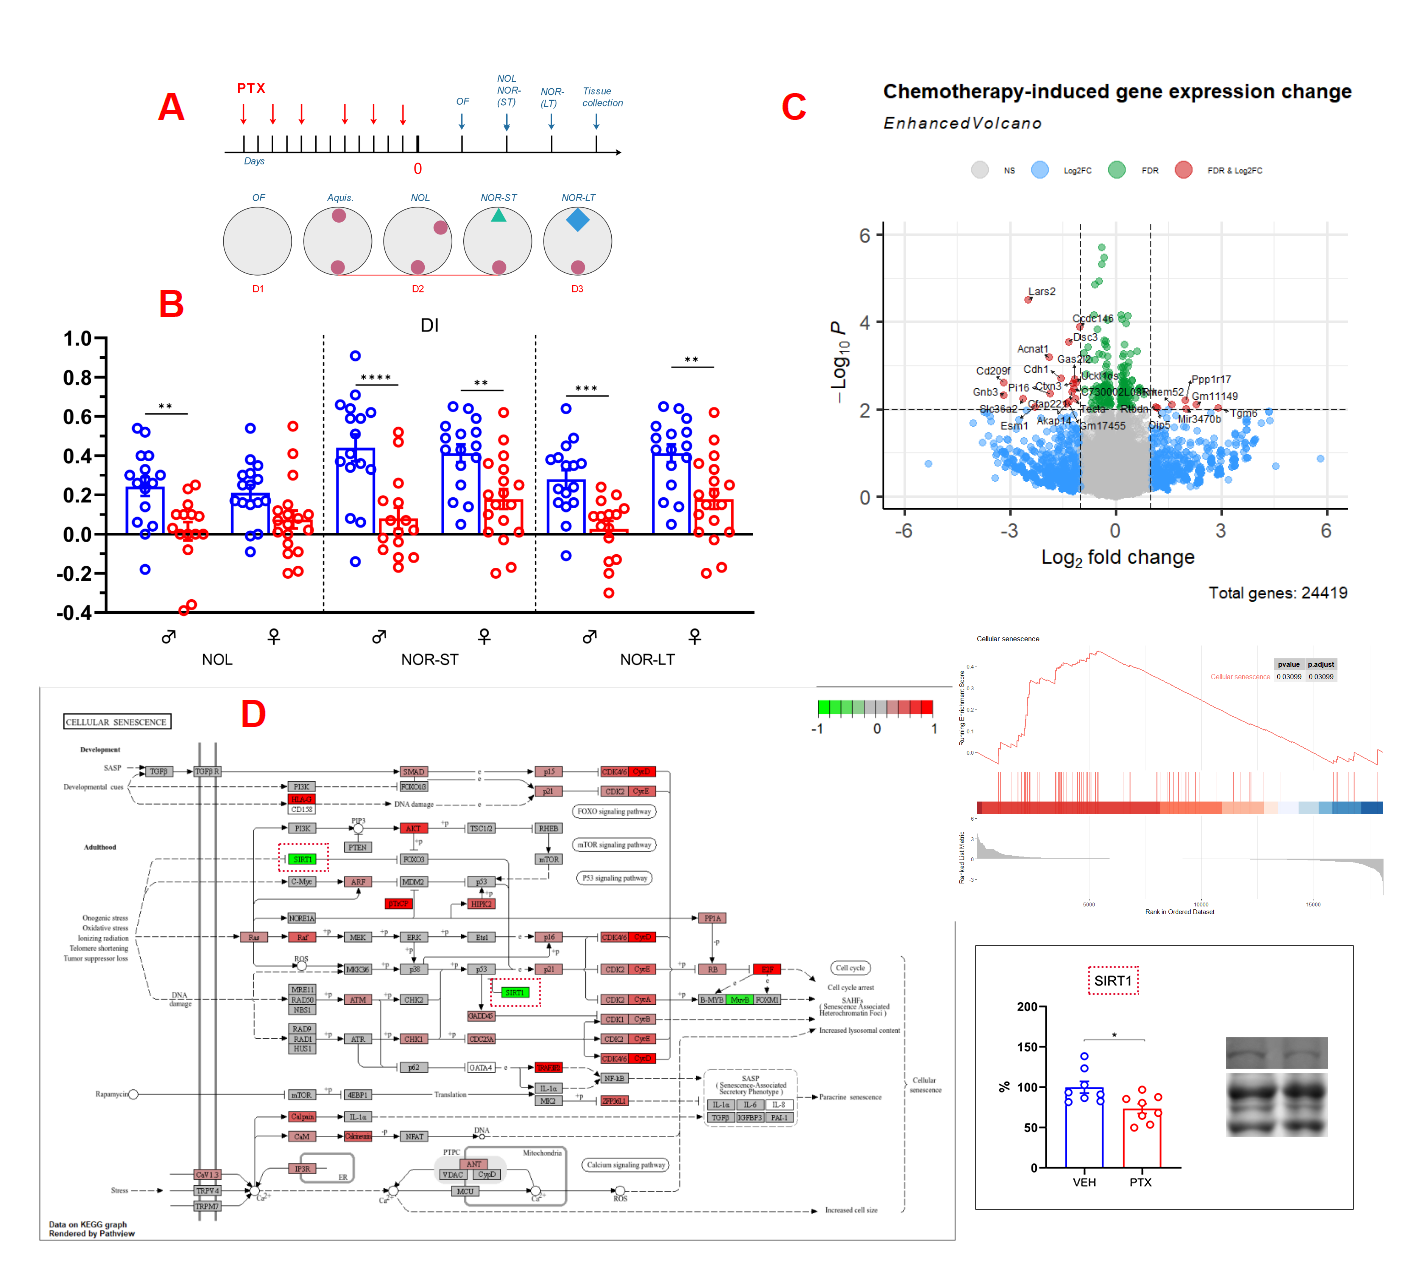
\includegraphics[height=12cm,keepaspectratio]{preliminary.png} % ou PD.pdf
	\caption{Resultados preliminares. A) Esquema de tratamento que será utilizado para indução do chemobrain durante a fase de validação dos resultados mais os ensaios comportamentais a serem realizados. B) Resultados de ensaios anteriores realizados pelo autor mostrando que o modelo de tratamento de fato induz o déficit cognitivo nos ensaios de Localização e reconhecimento de Objeto (Curto e longo prazo). B) Exemplo de resultado da análise de um Dataset de RNA seq bulk proveniente de hipocampo de animais tratados vs. não tratados com quimioterapia - Cavalier et al (2021). D) O conjunto de genes diferencialmente expressos mostrou-se associado significativamente com o fenótipo de senescência celular. Á direita, resultado de um Wester Blot realizado em nosso laboratório confirmando que um dos fatores (SIRT1), é alterado também a nível de proteína.}
	\label{fig:PD}
\end{figure} \indent 

	\newpage

	% ----------------------------
	% Referências
	% ----------------------------
	
	\printbibliography[title={Referências Bibliográficas}]
	
\end{document}